\documentclass[12pt,a4paper]{jsarticle}
\usepackage{amsmath}
\usepackage[dvipdfmx]{graphicx}
\everymath{\displaystyle}
\begin{document}
復習問題
\begin{enumerate}
    \item $\lim_{n\to \infty}a_n$の定義をかいてください。
    \\ヒント:無限個の足し算はできないので、有限和の極限と定義していました。\everymath{\displaystyle}
    \item $\sum_{k=1}^n \left(\frac{1}{3}\right)^k$
    \item $\sum_{n=1}^\infty \left(\frac{1}{3}\right)^n$
    \item $\frac{1}{1\cdot 3}+\frac{1}{2\cdot 4}+\frac{1}{3\cdot 5}+\cdots +\frac{1}{n\cdot (n+2)}$
    \item $\frac{1}{1\cdot 3}+\frac{1}{2\cdot 4}+\frac{1}{3\cdot 5}+\cdots$
\end{enumerate}
下のグラフはあとで使います\\
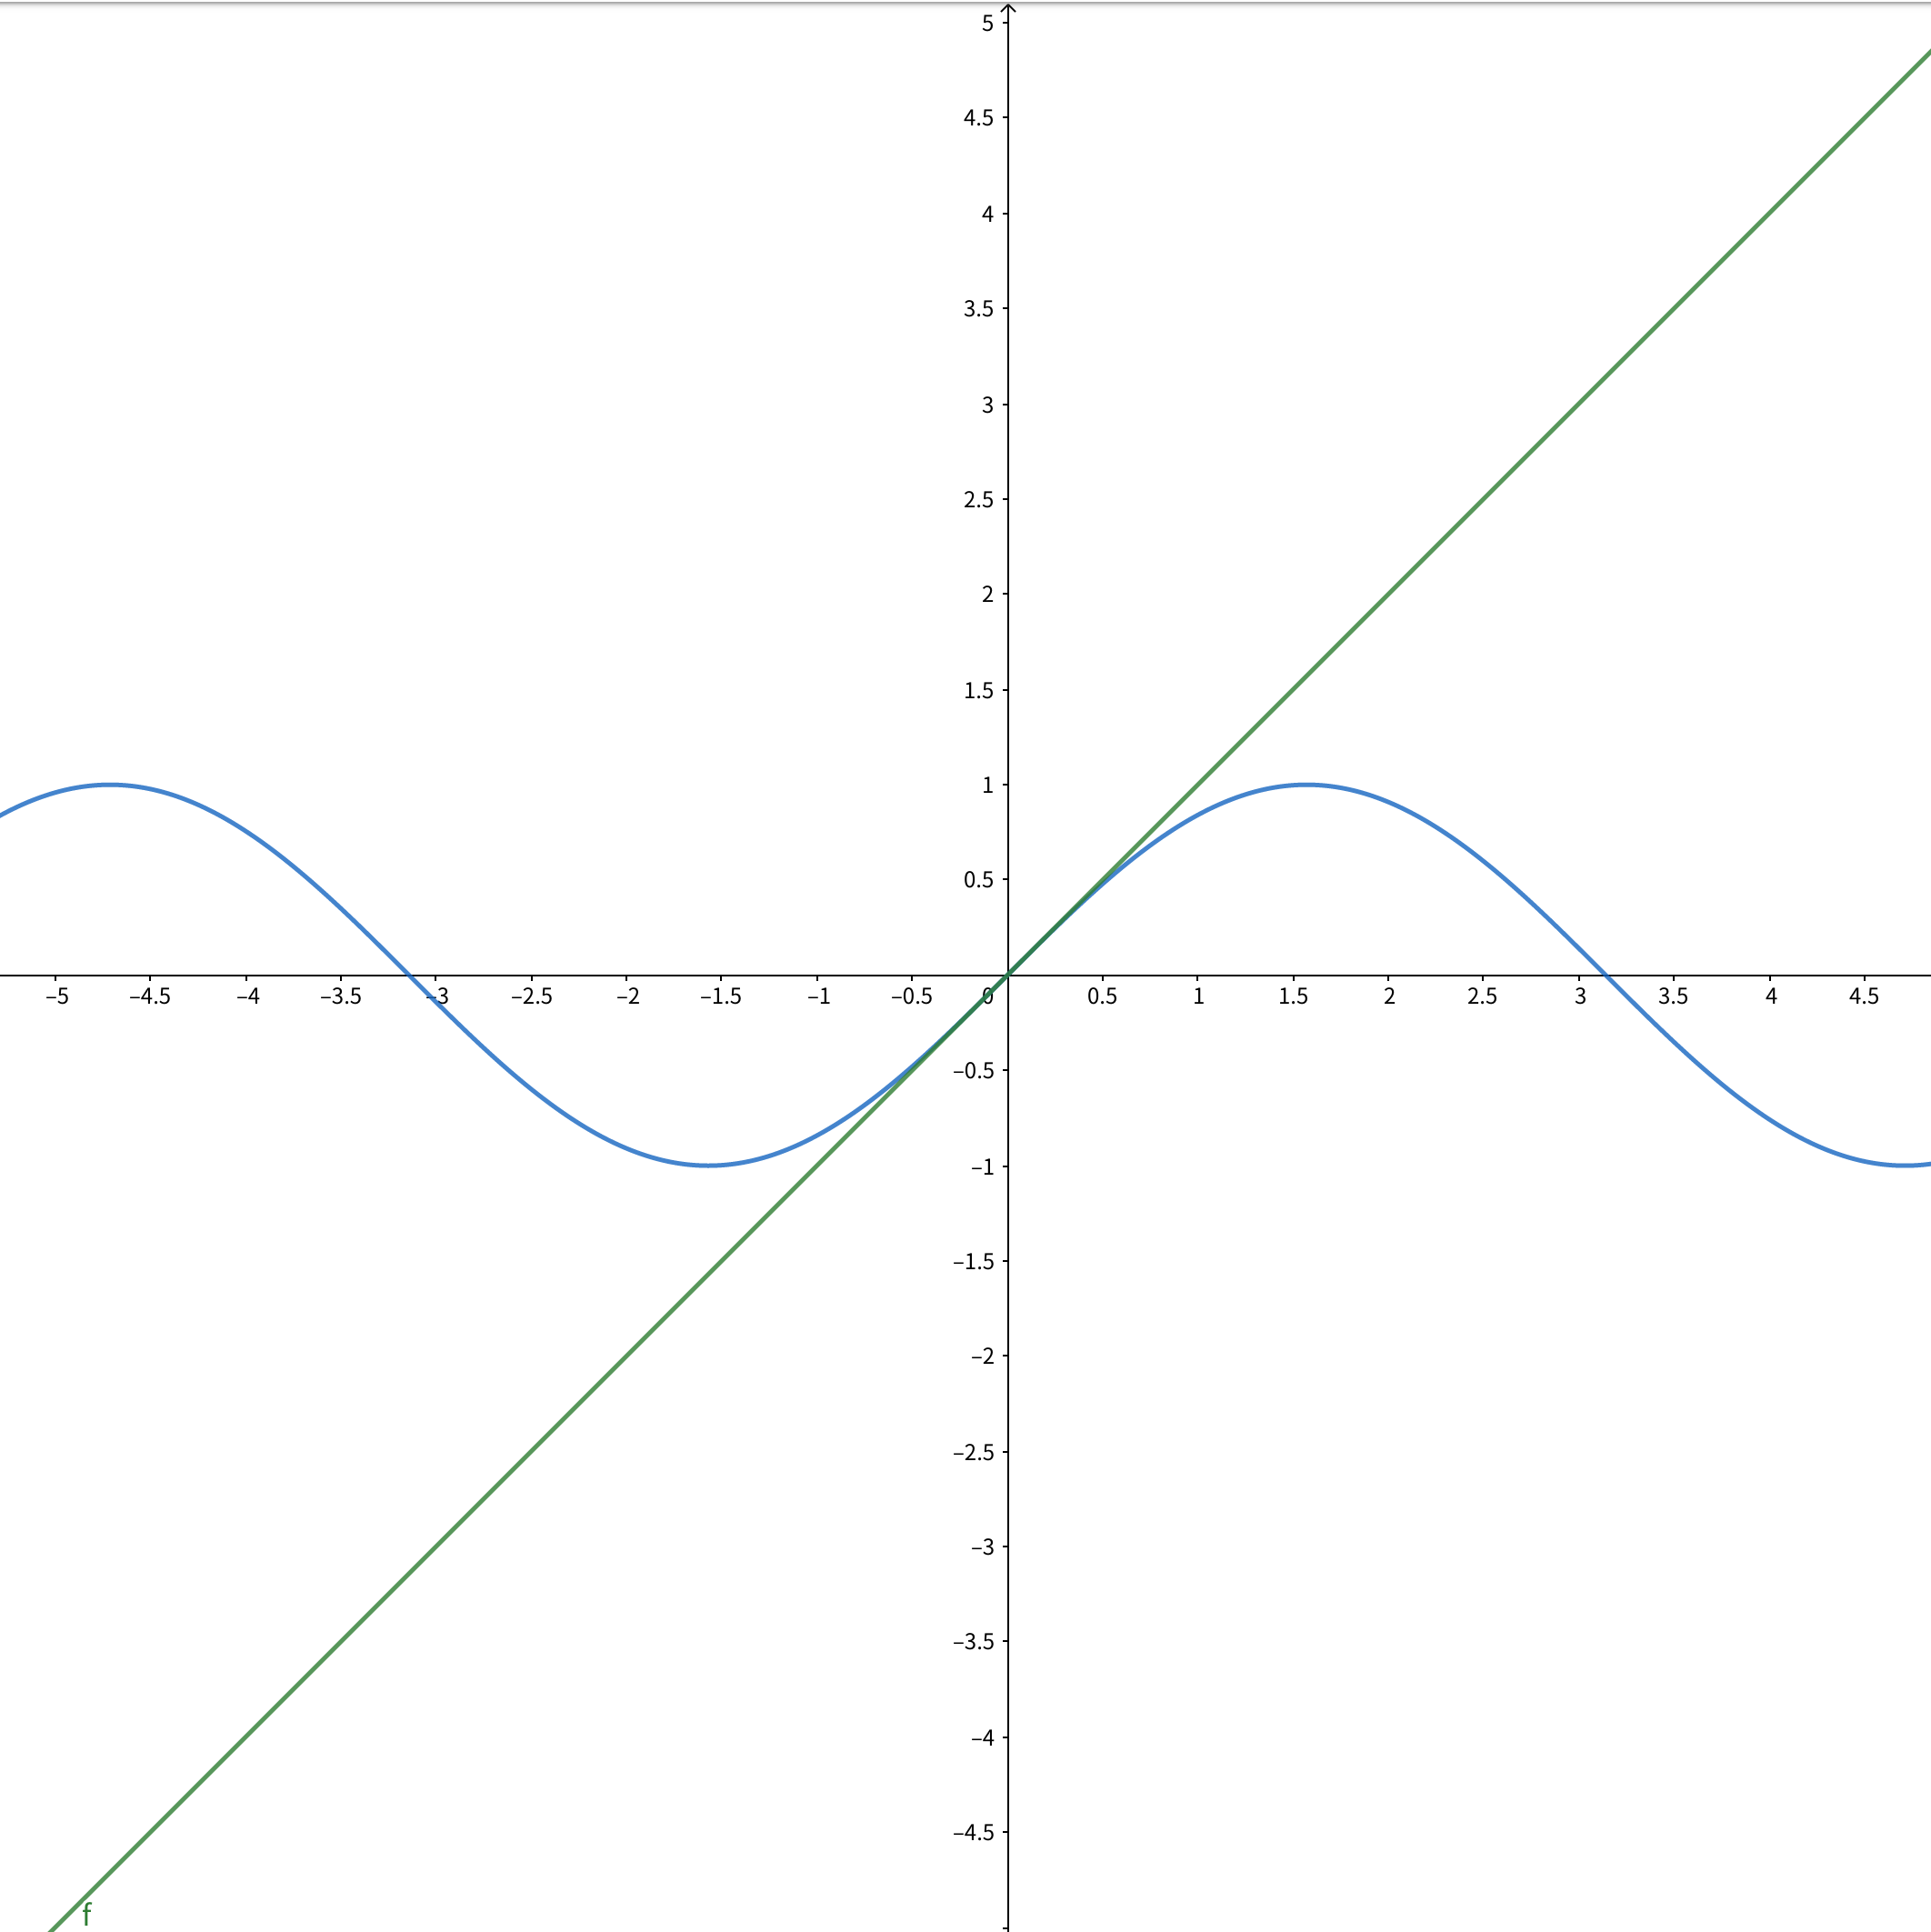
\includegraphics[width=5cm]{graphs/x-and-sin.png}
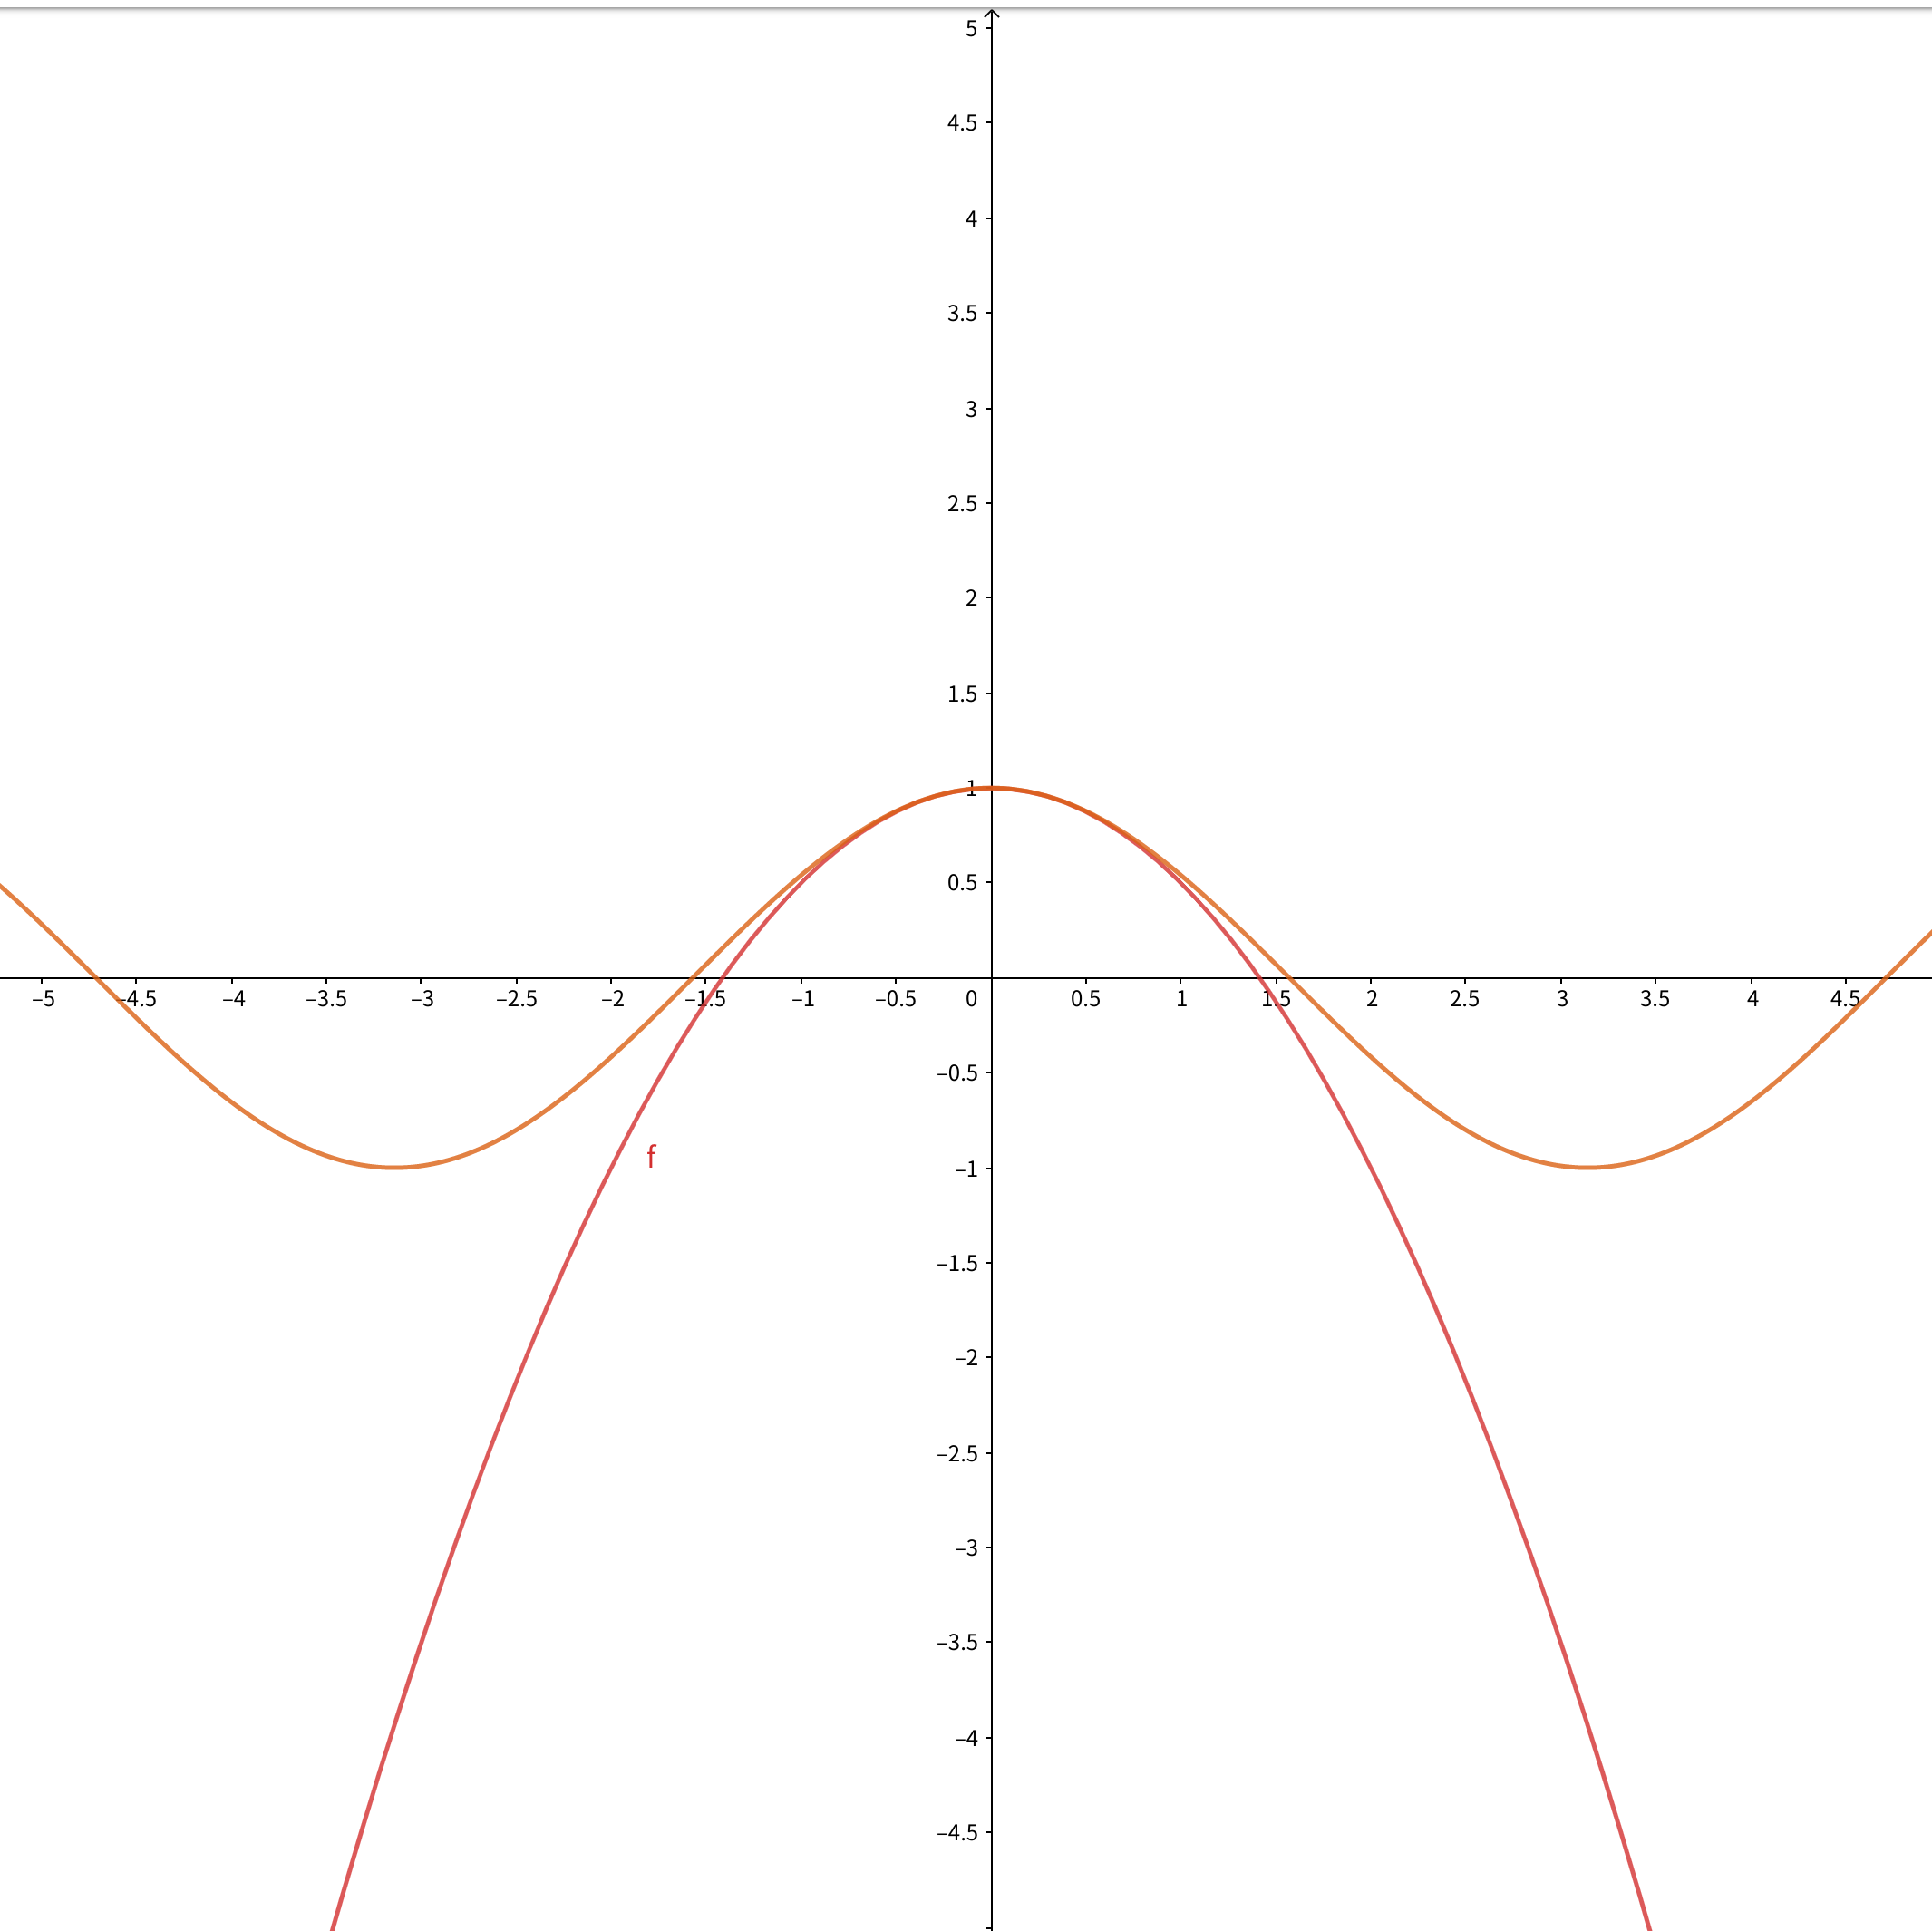
\includegraphics[width=5cm]{graphs/x2-and-cos.png}
\end{document}